\documentclass[xcolor=dvipsnames,10pt]{beamer}
% ********** Styl prezentacji **********
\mode<presentation>
{
%\usetheme{Frankfurt}
%\usetheme{Copenhagen}
\usetheme{Madrid}
 %\usetheme{lankton-keynote}
 %Copenhagen
}
%\usepackage{amsmath}
%\usepackage{amsthm}
%\usepackage{amsfonts}
\usepackage{color}
%\usepackage{listings}
%\lstset{language=C++}
%\usepackage{lscape} 
%\usepackage{float}
%\usepackage{graphicx}
\usepackage{caption}
\usepackage{subcaption}
%\usepackage{multimedia}
% common reference commands
\newcommand{\eqt}[1]{Eq.~(\ref{#1})}                     % equation
\newcommand{\fig}[1]{Fig.~\ref{#1}}                      % figure
\newcommand{\tbl}[1]{Table~\ref{#1}}                     % table
%\usepackage{movie15}
%\usepackage{hyperref}
%\usepackage{multimedia}
\usepackage[]{media9}
%\usepackage{filecontents,hyperref,listings}
\renewcommand{\div}{\vec{\nabla} \cdot}
\newcommand{\grad}{\vec{\nabla}}
%
%\setbeamertemplate{footline}[frame number]
%\title{Extension of the entropy viscosity method to low Mach regime and the seven equations model.}
%\title{Extension of the entropy viscosity method to low Mach regime and the seven equations model.}
%\author{Marc-Olivier Delchini}
%
\begin{document}
%
%\begin{frame}
%\maketitle
%\end{frame}
\begin{frame}
\centering
\begin{block}{\centering Application of the entropy viscosity method to the $1$-D grey Radiation-Hydrodynamic equations (RHD).}
\end{block}
\begin{center}
Marc-Olivier Delchini, Jim Morel and Jean Ragusa \\
\today
\end{center}
\begin{figure}[H]
        \centering
%        \begin{subfigure}[b]{0.4\textwidth}
                \centering
                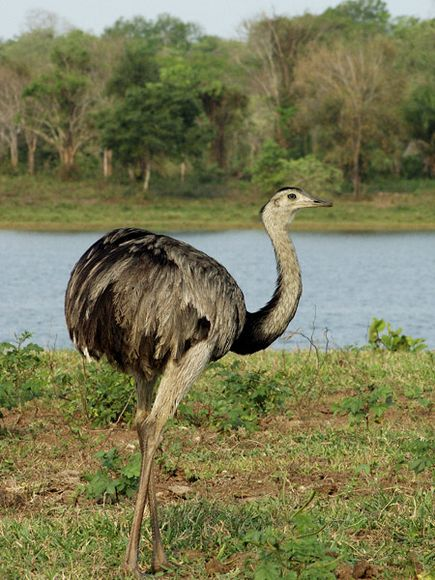
\includegraphics[width=0.35\textwidth]{rhea.png}
                \caption{Rhea}
\end{figure}%
\end{frame}
%
\begin{frame}
	\frametitle{Outline:}
	\tableofcontents
\end{frame}
%************************************************
\section{Objective and background.}
\begin{frame}{}
\begin{block}{Objective:}
Apply the entropy viscosity method to the $1$-D grey radiation-hydrodynamic equations $\rightarrow$ multiphysics problem with source terms.
\end{block}
\begin{block}{Background:}
\begin{itemize}
\setlength{\itemsep}{15pt}
\item RHD are a wave-dominated problem with source terms.
\item They are known to develop shocks due to the nature of Euler equations.
\item Great amount of work available in the literature on how to solve RHD: approximate Riemann solver \cite{LowrieMorel, Balsara}, flux limiter \cite{EdwardsMorelKnoll}, $\cdots$
\item Have a common approach: focus on the hyperbolic part of the RHD.
\item Attempts to derive a Riemann solver accounting for the source terms.
\item Use of semi-implicit schemes because of the difference of characteristic time scale between the two physics $\rightarrow$ implicit scheme has some advantage.
\end{itemize}
\end{block}
\end{frame}
%************************************************
\section{The $1$-D grey Radiation-Hydrodynamic equations (RHD).}
\begin{frame}{The $1$-D grey Radiation-Hydrodynamic equations (RHD):}
\begin{block}{RHD system of equations:}
\begin{align}
%\left\{
%\begin{array}{lll}
&\partial_t \left( \rho \right) + \partial_x\left( \rho u \right) = 0 \nonumber\\
&\partial_t \left( \rho u\right) + \partial_x \left(\rho u^2 + P  \right) = {\color{blue}-\partial_x \left(\frac{\epsilon}{3}\right)} \nonumber\\
&\partial_t \left( \rho E\right) + \partial_x \left[ u \left( \rho E + P \right) \right] = {\color{blue}-\frac{u}{3} \partial_x \epsilon - \sigma_a c \left( a T^4 - \epsilon \right)} \nonumber\\
&\partial_t \epsilon + \frac{4}{3} \partial_x \left( u \epsilon \right) = {\color{blue}\frac{u}{3} \partial_x \epsilon} + {\color{magenta}\partial_x \left( \frac{c}{3 \sigma_t} \partial_x \epsilon \right)} + {\color{blue}\sigma_a c \left( a T^4 - \epsilon \right)} \nonumber
%\end{array}
%\right. 
\nonumber
\end{align}
\end{block}
\begin{block}{A few remarks:}
\begin{itemize}
\setlength{\itemsep}{10pt}
\item Relaxation term in the energy and radiation equations: ${\color{blue}\sigma_a c \left( a T^4 - \epsilon \right)}$.% behaves like a diffusion term when $\sigma_a \to \infty$ \cite{ShiJin}.
\item Diffusion term: ${\color{magenta}\partial_x \left( \frac{c}{3 \sigma_t} \partial_x \epsilon \right)}$.
\item The above system of equations is NOT hyperbolic ???? 
\end{itemize}
\end{block}
\end{frame}
%************************************************
\begin{frame}{The entropy viscosity method (EVM) \cite{jlg}:}
\emph{It is an artificial dissipation method with smart viscosity coefficient(s)  capable of tracking the shock so that dissipation is only added into the shock region.}
\begin{block}{}
\begin{itemize}
\setlength{\itemsep}{15pt}
\item The method requires a \emph{hyperbolic system of equations}.
\item Add artificial dissipative terms consistent with the entropy minimum principle.
\item Define a local and smooth viscosity coefficient function of the grid size.
\item The viscosity coefficient is defined proportional to the entropy production.
\item The entropy production is locally computed by evaluating the entropy residual:
\begin{equation}
R_e = \partial_t s + \vec{u} \cdot \grad s \geq 0 \nonumber
\end{equation}
\end{itemize}
\end{block}
\end{frame}
%************************************************
\section{The theoretical approach.}
\begin{frame}{}
\begin{block}{Our approach:}
\begin{itemize}
\setlength{\itemsep}{10pt}
\item Consider the hyperbolic parts of the system of equations (no source terms).
\item Keep in mind that the source terms may affect the entropy viscosity method and their effect will have to be studied later.
\end{itemize}
\end{block}
\begin{block}{Our hyperbolic system of equations:}
\begin{equation}
\left\{
\begin{array}{lll}
\partial_t \left( \rho \right) + \partial_x\left( \rho u \right) = 0 \\
\partial_t \left( \rho u\right) + \partial_x \left(\rho u^2 + P + \frac{\epsilon}{3} \right) = 0 \\
\partial_t \left( \rho E\right) + \partial_x \left[ u \left( \rho E + P \right) \right] = 0 \\
\partial_t \epsilon + \frac{4}{3} \partial_x \left( u \epsilon \right) - \frac{u}{3} \partial_x \epsilon = 0
\end{array}
\right. 
\nonumber
\end{equation}
Eigenvalues: $\lambda_1 = u - c$, $\lambda_{2,3} = u$ and $\lambda_4 = u + c$ where $c$ is the speed of sound defined as:
\begin{equation}
c^2 =  \underbrace{P_{\rho} + \frac{P}{\rho^2}P_e}_{c^2_{\text{Euler}}} + \underbrace{ \frac{4 \epsilon}{9\rho}}_{c^2_{\text{rad}}} \nonumber
\end{equation}
\end{block}
\end{frame}
%************************************************
\begin{frame}
\begin{block}{Viscous regularization and viscosity coefficient(s):}
\begin{enumerate}
\setlength{\itemsep}{15pt}
\item Derive the dissipative terms using the modified system of equations (no source term). \\
An entropy $s$ function of the material density $\rho$ and internal energy $e$, and the radiation density energy $\epsilon$.
\item Define the viscosity coefficient(s).
\end{enumerate}
\end{block}
\begin{block}{Method of Manufactured Solutions and $1$-D results:}
\begin{enumerate}
\setlength{\itemsep}{15pt}
\item Study the effect of the source terms, $\partial_x \left( \frac{c}{3 \sigma_t} \partial_x \epsilon \right)$ and $\sigma_a c \left( a T^4 - \epsilon \right)$, on the entropy viscosity method using the Method of Manufactured Solutions (MMS), and show high-order convergence.
\item Perform $1$-D tests for different Mach numbers: Mach$=1.05$, $1.2$, $2$, $5$, and $50$. Semi-analytical solutions are available.
\end{enumerate}
\end{block}
\end{frame}
%************************************************
\subsection{A viscous regularization for the RHD}
\begin{frame}{}
\begin{block}{A viscous regularization for the RHD:}
\begin{align}
&\partial_t \left( \rho \right) + \partial_x\left( \rho u \right) = {\color{red}\partial_x \left( \kappa \partial_x \rho \right)} \nonumber \\
&\partial_t \left( \rho u \right) + \partial_x \left(\rho u^2 + P + \frac{\epsilon}{3} \right) = {\color{red}\partial_x \left( \mu \partial_x u \right) + \partial_x \left( \kappa \partial_x \rho \right)} \nonumber \\
&\partial_t \left( \rho E\right) + \partial_x \left[ u \left( \rho E + P \right) \right] = {\color{red}\partial_x \left( \kappa \partial_x \rho e \right) + 0.5 \partial_x \left( \kappa u^2 \partial_x \rho \right) + \partial_x \left( \mu \rho u  \partial_x u \right)} \nonumber \\
&\partial_t \epsilon + \frac{4}{3} \partial_x \left( u \epsilon \right) - \frac{u}{3} \partial_x \epsilon = {\color{red}\partial_x \left( \kappa \partial_x \epsilon \right)} \nonumber
\end{align}
\end{block}
\begin{block}{The entropy inequality:}
\begin{equation}
R_e = \partial_t s + u \partial_x s = \frac{s_e}{P_e} \underbrace{\left( \frac{DP}{Dt} - c^2_{Euler} \frac{D\rho}{Dt} \right)}_{\tilde{R}_e} \geq 0 \nonumber
\end{equation}
where $s(\rho,e,\alpha) = s_{Euler}(\rho, e) + \frac{\rho_0}{\rho} \hat{s}(\alpha)$, $s_{Euler}$ and $\hat{s}$ being concave. 
\end{block}
\begin{block}{}
%\begin{itemize}
two viscosity coefficients: $\kappa$ and $\mu$. In the remaining of this presentation, we will assume that $\mu = \kappa$ $\rightarrow$ parabolic regularization.
%\end{itemize}
\end{block}
\end{frame}
%************************************************
\subsection{Definition of the viscosity coefficient.}
\begin{frame}{}
\begin{block}{Definition of the viscosity coefficient $\mu$:}
\begin{align}
&\mu(x,t) = \min \left( \mu_{max}(x,t), \mu_e(x,t) \right) \nonumber \\
&\mu_{max}(x,t) = 0.5 h \left( | u | + c \right) \nonumber \\
&\mu_e(x,t) = h^2 \frac{\max \left( \tilde{R}_e(x,t), J \right)}{norm_P} \nonumber
\end{align}
\end{block}
\begin{block}{Entropy residual:}
\begin{equation}
\tilde{R}_e =  \frac{DP}{Dt} - c^2_{Euler} \frac{D\rho}{Dt} \nonumber
\end{equation}
\end{block}
\begin{block}{The jump $J$ and the normalization parameter $norm_P$:}
\begin{align}
&J = \max \left(| u |  [[\partial_x P]],  |u| c_{Euler}^2 [[\partial_x \rho]] \right) \nonumber \\
&norm_P = \rho c_{Euler}^2 \nonumber
\end{align}
\end{block}
\end{frame}
%************************************************
\begin{frame}{}
\begin{block}{EVM and the diffusion term $\partial_x \left( \frac{c}{3 \sigma_t} \partial_x \epsilon \right)$:}
In the radiation equation, there are two second-order terms: diffusion and dissipative terms.
\begin{align}
{\color{magenta}\partial_x \left( \frac{c}{3 \sigma_t} \partial_x \epsilon \right)} + {\color{red}\partial_x \left( \kappa \partial_x \epsilon \right)} \rightarrow \partial_x \left( \max \left( {\color{magenta}\frac{c}{3 \sigma_t}} , {\color{red}\kappa} \right) \partial_x \epsilon \right) \nonumber
\end{align}
\end{block}
\end{frame}
%************************************************
\begin{frame}{EVM and the relaxation term}
\begin{block}{Relaxation term:}
\begin{equation}
\left\{
\begin{array}{ll}
\partial_t u + \partial_x v = 0 \nonumber \\
\partial_t v + \partial_x p(u) = \frac{1}{\psi} \left( v - f(u) \right) \nonumber
\end{array}
\right.
\end{equation}
as $\psi \to 0$, it can be shown that:
\begin{equation}
\left\{
\begin{array}{ll}
v \sim f(u) \nonumber \\
\partial_t u + \partial_x f(u) = \partial_x \left( \beta \partial_x u \right) \nonumber
\end{array}
\right.
\end{equation}
where $\beta$ is function of $\psi$, $p(u)$ and $f(u)$.
\end{block}
\begin{block}{Problem:}
$\Rightarrow$ the relaxation term behaves as a diffusion term in the asymptotic limit and thus, will compete with the dissipative term.
\end{block}
\begin{block}{Solution:}
MMS to investigate the behavior of the dissipative terms in the asymptotic limit.
\end{block}
\end{frame}
%************************************************
\begin{frame}{The code}
\begin{block}{}
\begin{itemize}
\setlength{\itemsep}{15pt}
\item Idaho National Laboratory MOOSE framework.
\item Fully implicit $\rightarrow$ non-linear solver with a preconditioner.
\item Continuous Galerkin Finite Element Method (CGFEM).
\item Second-order accuracy in time (BDF2) and space (linear polynomials).
\item Gauss quadrature rule.
\item RHEA: Radiation-Hydrodynamic EquAtions ($1$-D code). 
\end{itemize}
\end{block}
\end{frame}
%************************************************
\begin{frame}{}
\begin{block}{MMS: the equilibrium diffusion limit}
\begin{align}
& \rho = \sin (x-t)+2 \nonumber \\
& u = \cos(x-t) +2 \nonumber \\
& T = \frac{0.5 \gamma (\cos(x-t) +2) }{\sin (x-t)+2}\nonumber \\
& \epsilon = a T^4 \nonumber 
\end{align}
\end{block}
$\sigma_a = \sigma_t = 1000$ $cm^{-1}$.
\end{frame}
%************************************************
\begin{frame}{}
\begin{table}[H]
\caption{L$_2$ norms of the error for for the equilibrium diffusion limit case using a manufactured solution.}
\begin{center}
\resizebox{\columnwidth}{!}{
\begin{tabular}{|c|c|c|c|c|c|c|c|c|c|}
\hline
\textbf{\# of cells} & time step size $(sh)$  & $\mathbf{\rho}$ & \textbf{ratio} & $\mathbf{\rho E}$ & \textbf{ratio} \\ \hline
$20$ & $10^{-1}$ &	 $0.590766$ & NA &  $1.333774$ & NA \\ \hline
$40$ & $5$ $10^{-1}$ & $0.290626$ & $2.03$ &  $0.478819$ & $2.79$ \\ \hline
$80$ & $2.5$ $10^{-2}$ & $0.0959801$ & $3.021$ &  $0.154119$ & $3.11$ \\ \hline
$160$ & $1.25$ $10^{-2}$ & $0.02593738$ & $3.70$ &  $0.0405175$ & $3.80$ \\ \hline
$320$ & $6.25$ $10^{-3}$ & $6.471444$ $10^{-3}$ & $4.00$ & $9.90446$ $10^{-3}$ & $4.09$ \\ \hline
$640$ & $3.125$ $10^{-3}$ & $1.584158$ $10^{-3}$ & $4.01$ & $2.44727$ $10^{-3}$ & $4.04$ \\ \hline
\hline
\textbf{\# of cells} & time step size $(sh)$  & $\mathbf{\epsilon}$ & \textbf{ratio} &  $\mathbf{\rho u}$ & \textbf{ratio} \\ \hline
$20$ & $10^{-1}$ &  $0.00650085$ & NA & $0.910998$ & NA	\\ \hline
$40$ & $5$ $10^{-1}$ &  $0.00124983$ & $5.20$ & $0.4090946$ & $2.23$	\\ \hline
$80$ & $2.5$ $10^{-2}$ &  $0.000262797$ & $4.76$ & $0.125943$ & $3.25$	\\ \hline
$160$ & $1.25$ $10^{-2}$ &  $6.17726$ $10^{-5}$ & $4.25$ & $3.381042$ $10^{-3}$ & $3.72$	\\  \hline
$320$ & $6.25$ $10^{-3}$ & $1.509184$ $10^{-5}$ & $4.09$ & $8.373657$ $10^{-3}$ & $4.04$ \\ \hline 
$640$ & $3.125$ $10^{-3}$  & $3.72548$ $10^{-6}$ & $4.05$ & $2.070538$ $10^{-3}$ & $4.04$ \\ \hline   
\end{tabular}  
}
\end{center}
\end{table}
\end{frame}
%************************************************
\begin{frame}
The second manufactured solution is used to test the method in the streaming limit: the radiation streaming dominates the absorption/re-emission term and evolves at a fast time scale.
\begin{block}{MMS: the streaming limit}
\begin{align}
&\rho = \sin(x-t)+2 \nonumber \\
&u = \left( \sin(x-t)+2 \right)^{-1} \nonumber \\
&T = 0.5 \gamma \nonumber \\
&\epsilon = \sin(x-1000 t)+2 \nonumber
\end{align}
\end{block}
$\sigma_a = \sigma_t = 1$ $cm^{-1}$.
\end{frame}
%************************************************
\begin{frame}
\begin{table}[H]
\begin{center}
\caption{ L$_2$ norms of the error for for the streaming limit case using a manufactured solution.}
\resizebox{\columnwidth}{!}{
\begin{tabular}{|c|c|c|c|c|c|}
\hline
\textbf{\# of cells} & time step size $(sh)$  & $\mathbf{\rho}$ & \textbf{ratio} & $\mathbf{\rho E}$ & \textbf{ratio} \\ \hline
$20$ &$10^{-1}$& $1.4373$ $10^{-2}$ & NA & $5.88521$ $10^{-1}$ & NA \\ \hline
$40$ & $5.$ $10^{-2}$& $3.760208$ $10^{-3}$ & $3.82$ & $1.4244$ $10^{-1}$ & $4.13$ \\ \hline 
$80$ & $2.5$ $10^{-2}$& $9.91724$ $10^{-4}$ & $3.79$ & $3.2047$ $10^{-2}$ & $4.44$  \\ \hline      
$160$ & $1.25$ $10^{-2}$ & $2.4455$ $10^{-4}$ & $4.06$ & $7.4886$ $10^{-3}$ & $4.28$  \\ \hline     
$320$ & $6.25$ $10^{-3}$ & $6.280715$ $10^{-5}$ & $3.89$ & $1.82327$ $10^{-3}$ & $4.11$ \\ \hline 
$640$ & $3.125$ $10^{-3}$ & $1.57920$ $10^{-5}$ & $3.98$ & $4.50463$ $10^{-4}$ & $4.05$  \\ \hline
$1280$ & $1.5625$ $10^{-4}$ & $3.96096$ $10^{-6}$ & $3.99$ & $1.12061$ $10^{-4}$ & $4.02$ \\ \hline
\hline
\textbf{\# of cells} & time step size $(sh)$  & $\mathbf{\epsilon}$ & \textbf{ratio} &  $\mathbf{\rho u}$ & \textbf{ratio} \\ \hline
$20$ &$10^{-1}$ & $3.82001$ $10^{-1}$ & NA & $2.354671$ $10^{-3}$ & NA \\ \hline
$40$ & $5.$ $10^{-2}$ & $1.21500$ $10^{-1}$ &$3.14$& $6.138814$ $10^{-4}$& $3.84$ \\ \hline
$80$ & $2.5$ $10^{-2}$ & $3.27966$ $10^{-2}$ &$3.70$& $1.74974$ $10^{-4}$ & $3.51$ \\ \hline
$160$ & $1.25$ $10^{-2}$ & $8.38153$ $10^{-3}$ &$3.91$& $3.61297$ $10^{-5}$  & $4.84$ \\ \hline
$320$ & $6.25$ $10^{-3}$ & $2.10925$ $10^{-3}$ &$3.97$& $9.03866$ $10^{-6}$ & $3.99$ \\ \hline
$640$ & $3.125$ $10^{-3}$ & $5.28472$ $10^{-4}$ &$3.99$& $2.25649$ $10^{-6}$ & $4.01$ \\ \hline
$1280$ & $1.5625$ $10^{-4}$ &$1.322268$ $10^{-4}$ &$3.99$& $5.69984$ $10^{-7}$ & $3.95$ \\ \hline
\end{tabular}
}
\end{center}
\end{table}
\end{frame}
%************************************************
\section{$1$-D numerical results}
\begin{frame}
\begin{block}{$1$-D numerical results:}
\begin{itemize}
\setlength{\itemsep}{15pt}
\item Inlet Mach number: $1.05$, $1.2$, $2$, $5$ and $50$.
\item Step initial conditions.
\item All tests reach a steady-state solution.
\item BDF2 and linear polynomials.
\item Uniform mesh.
\item Semi-analytical solutions are plotted for comparison.
\end{itemize}
\end{block}
\end{frame}
%************************************************
\begin{frame}{Numerical results: Mach $1.05$.}
\begin{figure}[H]
        \centering
        \begin{subfigure}[b]{0.4\textwidth}
                \centering
                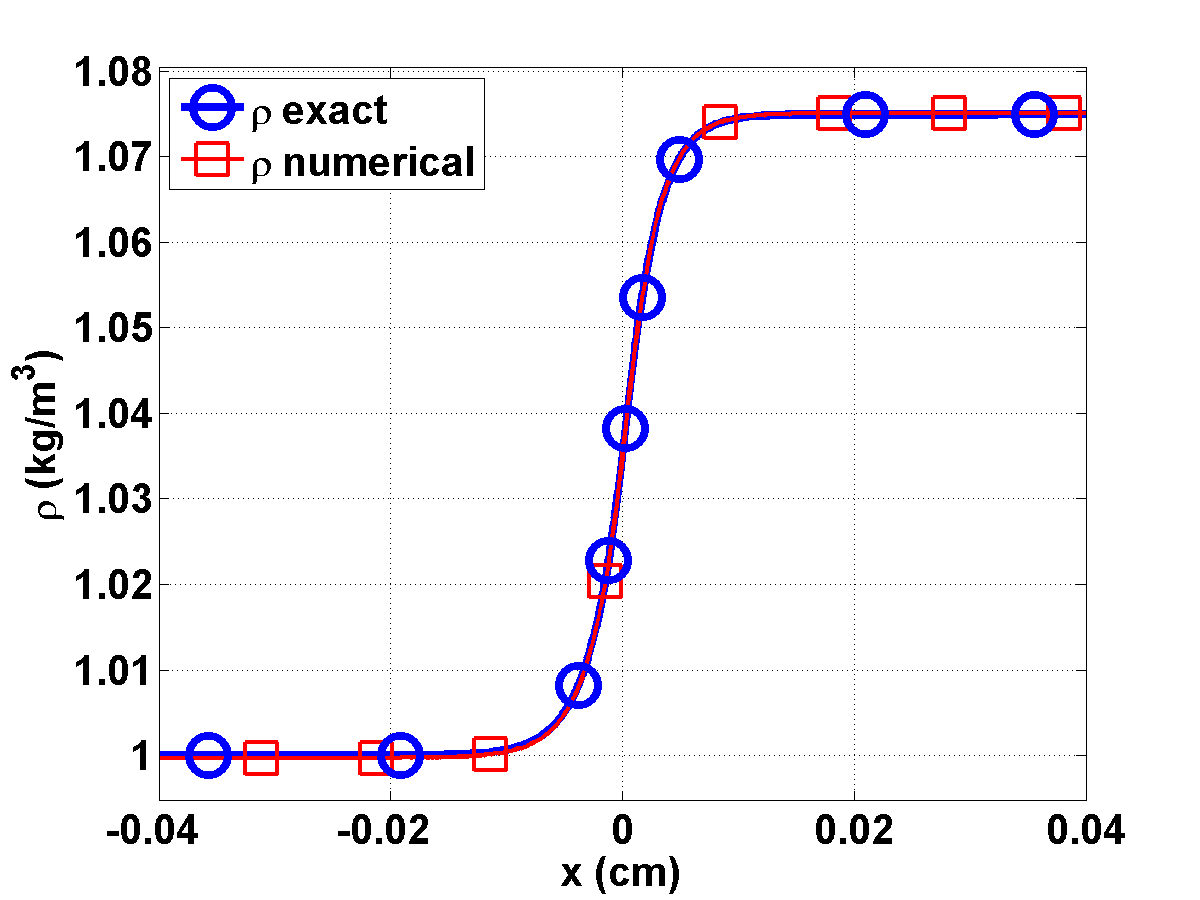
\includegraphics[width=\textwidth]{../elsarticle/Mach_1p05_nel_500_density.png}
%                \caption{Pressure}
        \end{subfigure}%
        ~ %add desired spacing between images, e. g. ~, \quad, \qquad etc. 
          %(or a blank line to force the subfigure onto a new line)
        \begin{subfigure}[b]{0.4\textwidth}
                \centering
                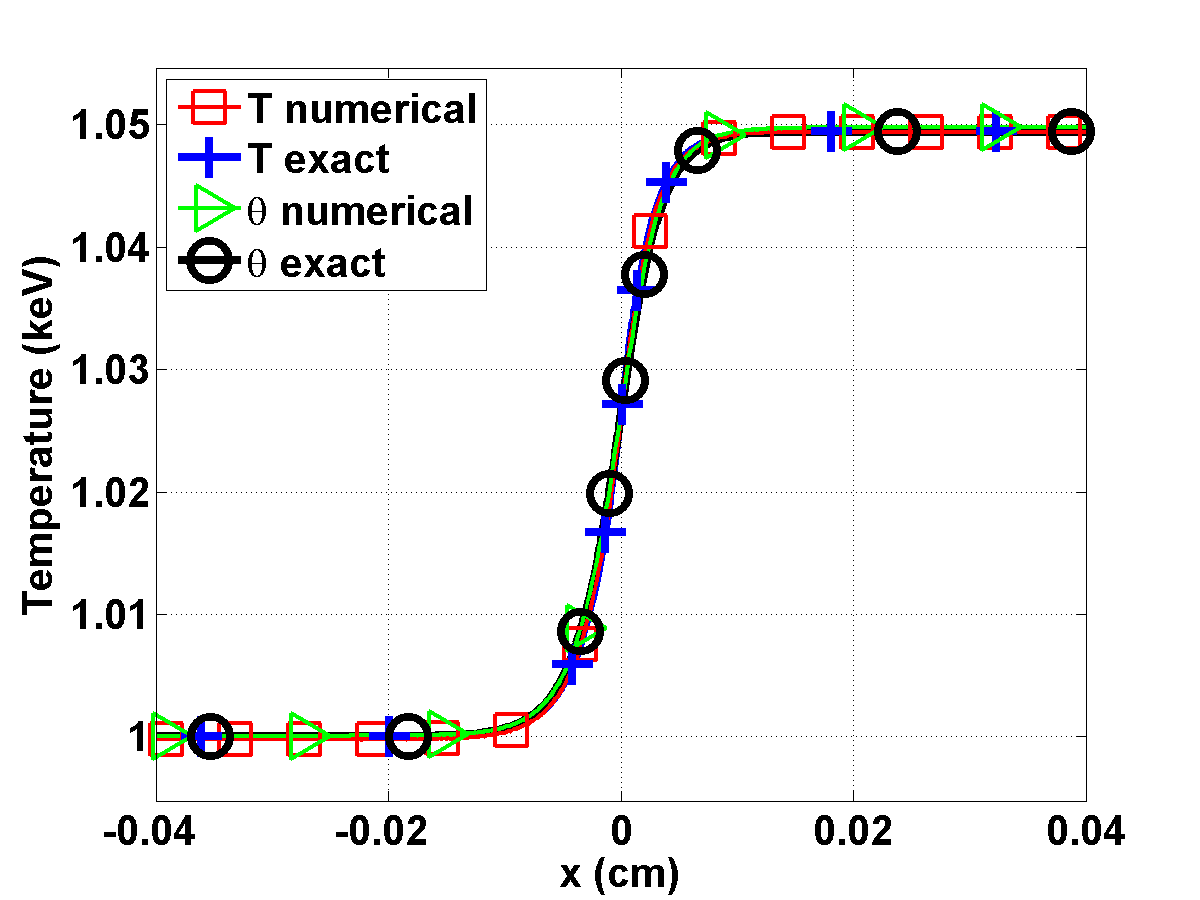
\includegraphics[width=\textwidth]{../elsarticle/Mach_1p05_nel_500_temperature.png}
%                \caption{Velocity.}
        \end{subfigure}
         %add desired spacing between images, e. g. ~, \quad, \qquad etc. 
          %(or a blank line to force the subfigure onto a new line)
        \begin{subfigure}[b]{0.4\textwidth}
                \centering
                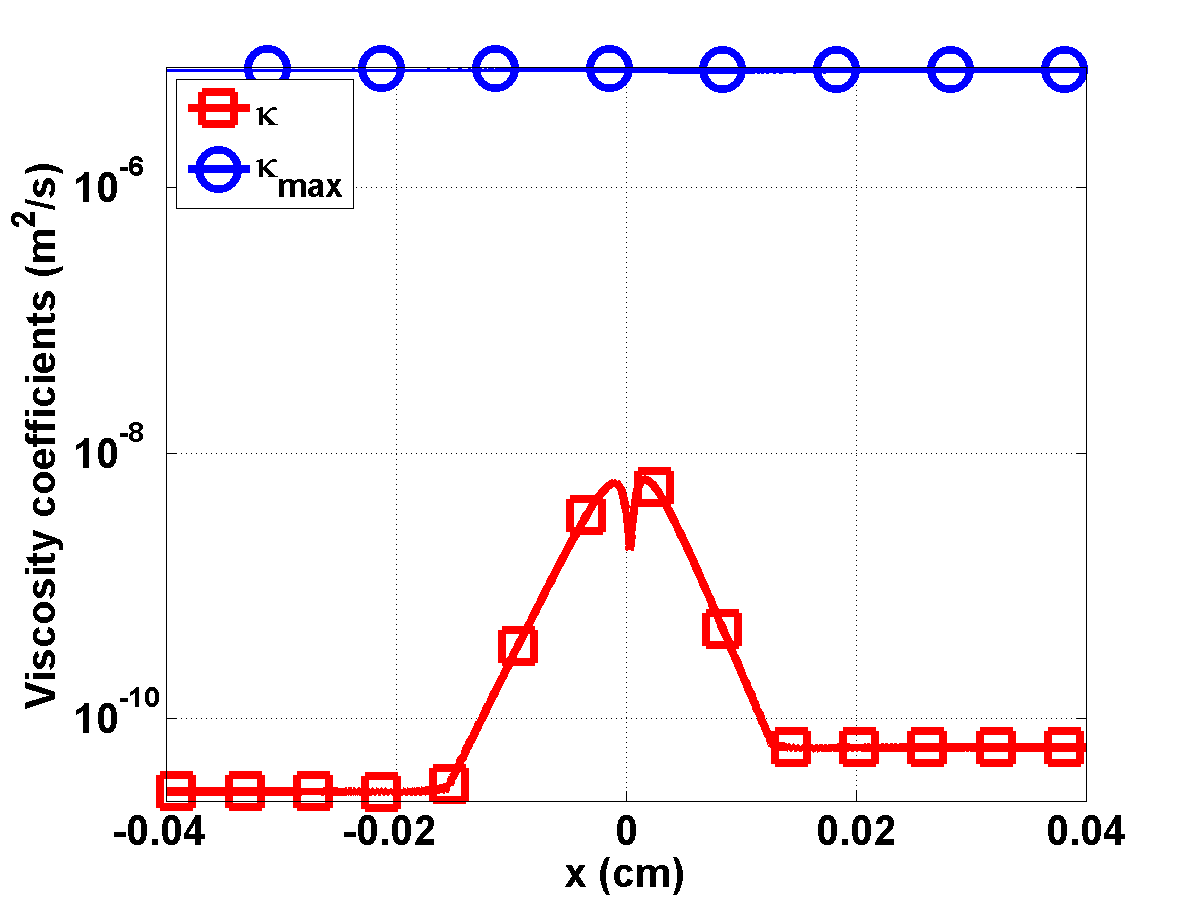
\includegraphics[width=\textwidth]{../elsarticle/Mach_1p05_nel_500_viscosity.png}
%                \caption{Density.}
        \end{subfigure}
        \caption{Steady-state numerical solution with $500$ cells, linear polynomials and BDF2.}
        \end{figure}
\end{frame}
%************************************************
\begin{frame}{Numerical results: Mach $1.2$.}
\begin{figure}[H]
        \centering
        \begin{subfigure}[b]{0.4\textwidth}
                \centering
                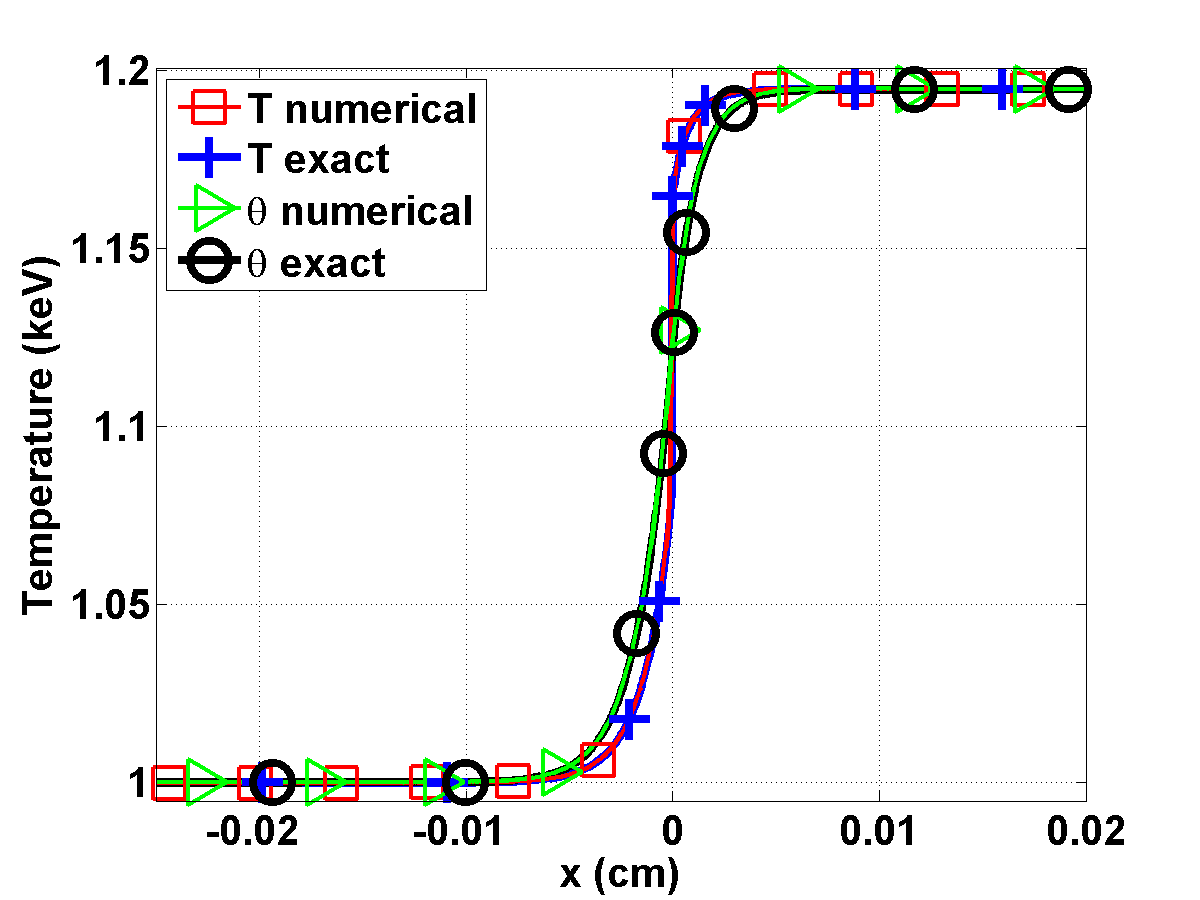
\includegraphics[width=\textwidth]{../elsarticle/Mach_1p2_nel_1000_temperature.png}
%                \caption{Pressure}
        \end{subfigure}%
        ~ %add desired spacing between images, e. g. ~, \quad, \qquad etc. 
          %(or a blank line to force the subfigure onto a new line)
        \begin{subfigure}[b]{0.4\textwidth}
                \centering
                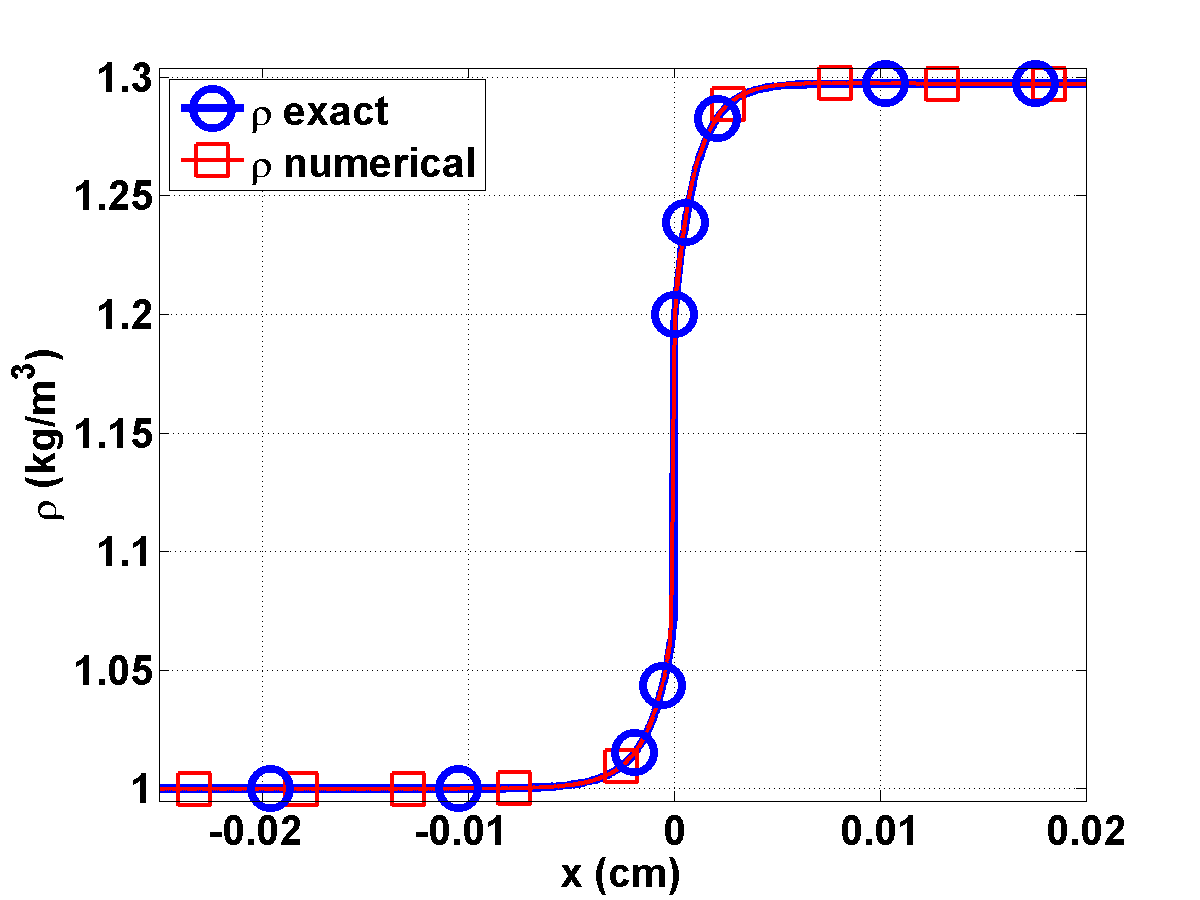
\includegraphics[width=\textwidth]{../elsarticle/Mach_1p2_nel_1000_density.png}
%                \caption{Velocity.}
        \end{subfigure}
         %add desired spacing between images, e. g. ~, \quad, \qquad etc. 
          %(or a blank line to force the subfigure onto a new line)
        \begin{subfigure}[b]{0.4\textwidth}
                \centering
                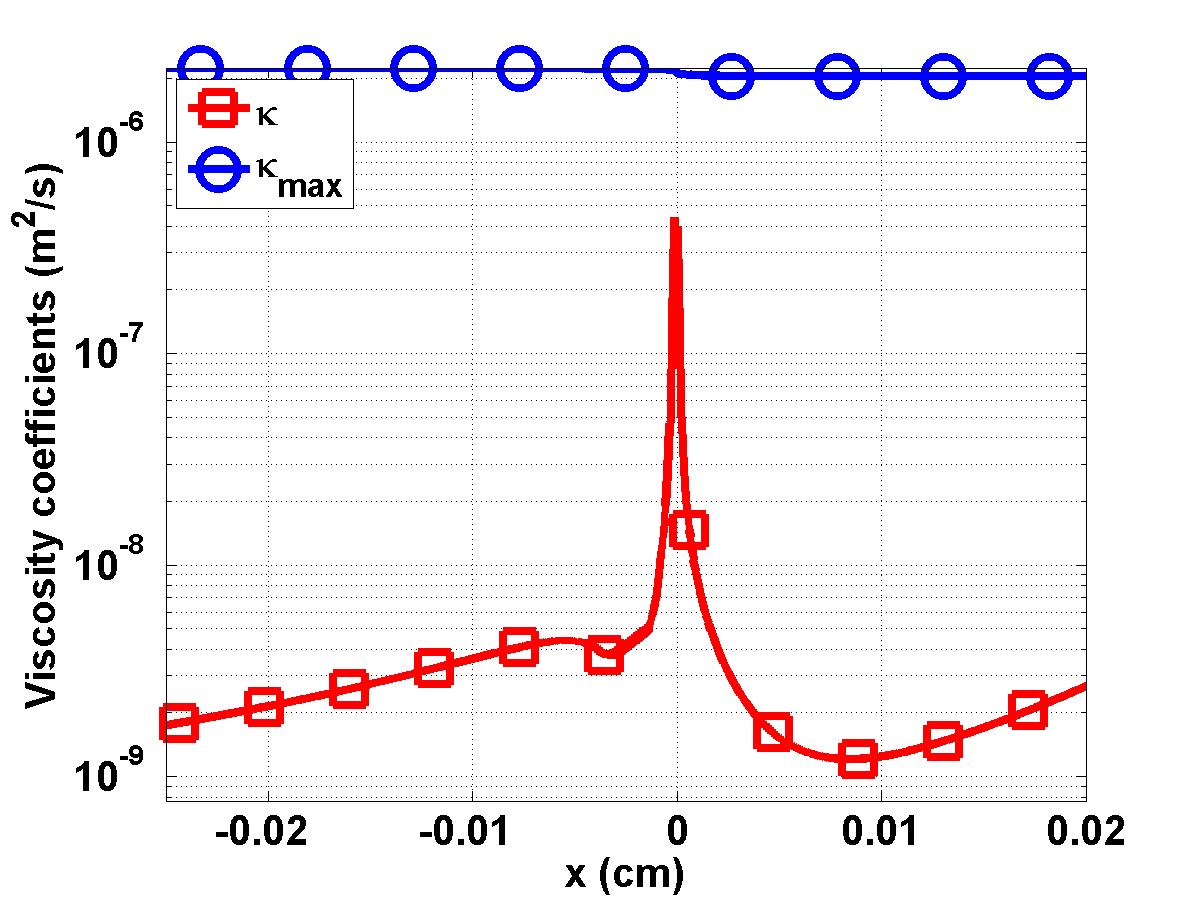
\includegraphics[width=\textwidth]{../elsarticle/Mach_1p2_nel_1000_viscosity.png}
%                \caption{Density.}
        \end{subfigure}
        \caption{Steady-state numerical solution with $1000$ cells, linear polynomials and BDF2.}
        \end{figure}
\end{frame}
%************************************************
\begin{frame}{Numerical results: Mach $2$.}
\begin{figure}[H]
        \centering
        \begin{subfigure}[b]{0.4\textwidth}
                \centering
                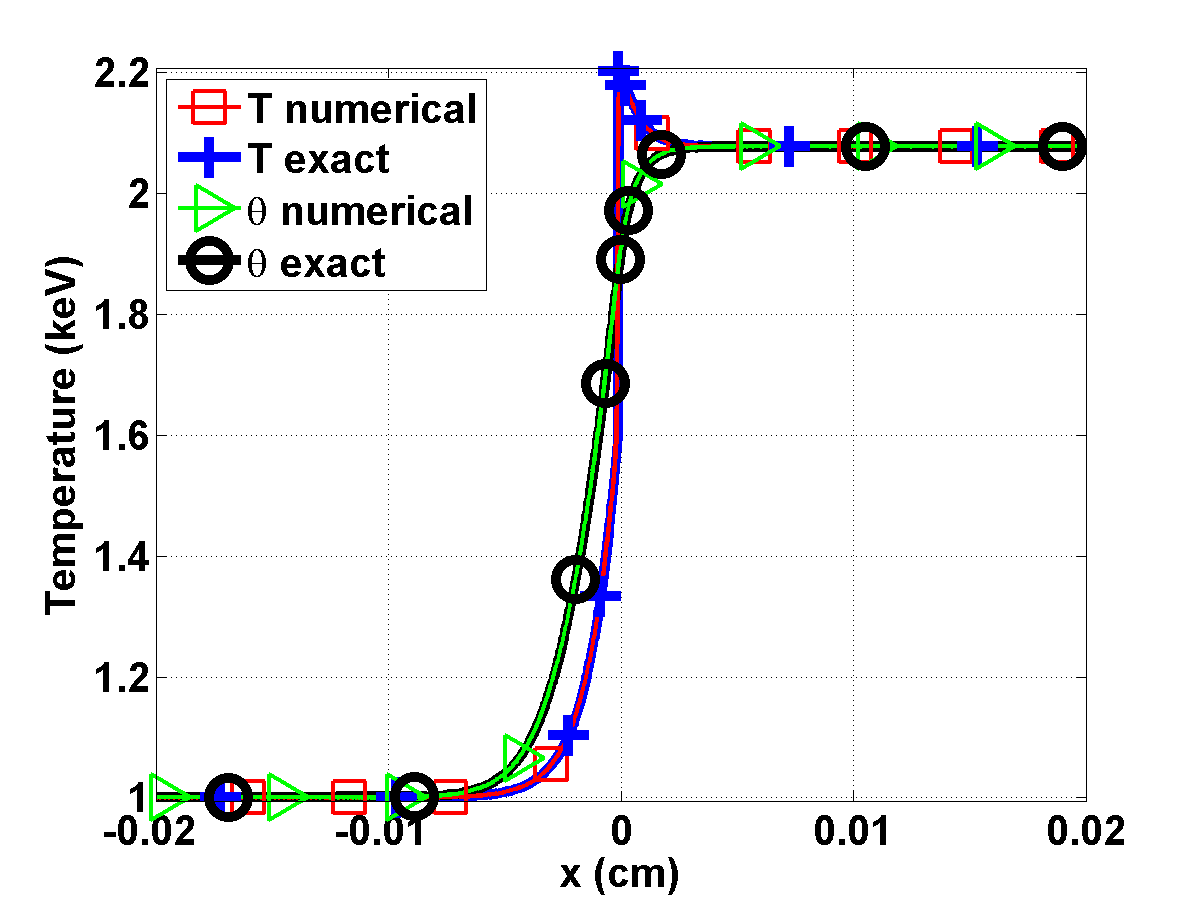
\includegraphics[width=\textwidth]{../elsarticle/Mach_2_nel_2000_temperature.png}
%                \caption{Pressure}
        \end{subfigure}%
        ~ %add desired spacing between images, e. g. ~, \quad, \qquad etc. 
          %(or a blank line to force the subfigure onto a new line)
        \begin{subfigure}[b]{0.4\textwidth}
                \centering
                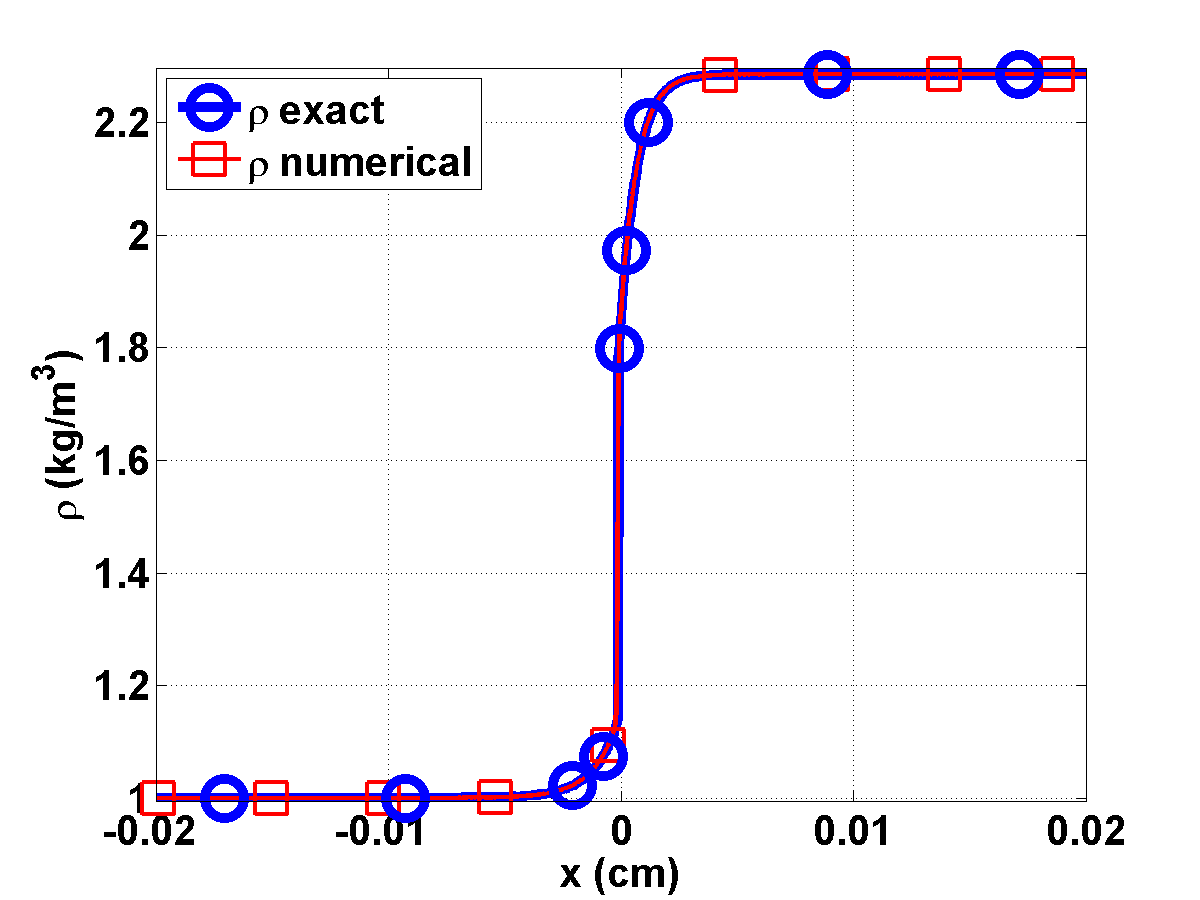
\includegraphics[width=\textwidth]{../elsarticle/Mach_2_nel_2000_density.png}
%                \caption{Velocity.}
        \end{subfigure}
         %add desired spacing between images, e. g. ~, \quad, \qquad etc. 
          %(or a blank line to force the subfigure onto a new line)
        \begin{subfigure}[b]{0.4\textwidth}
                \centering
                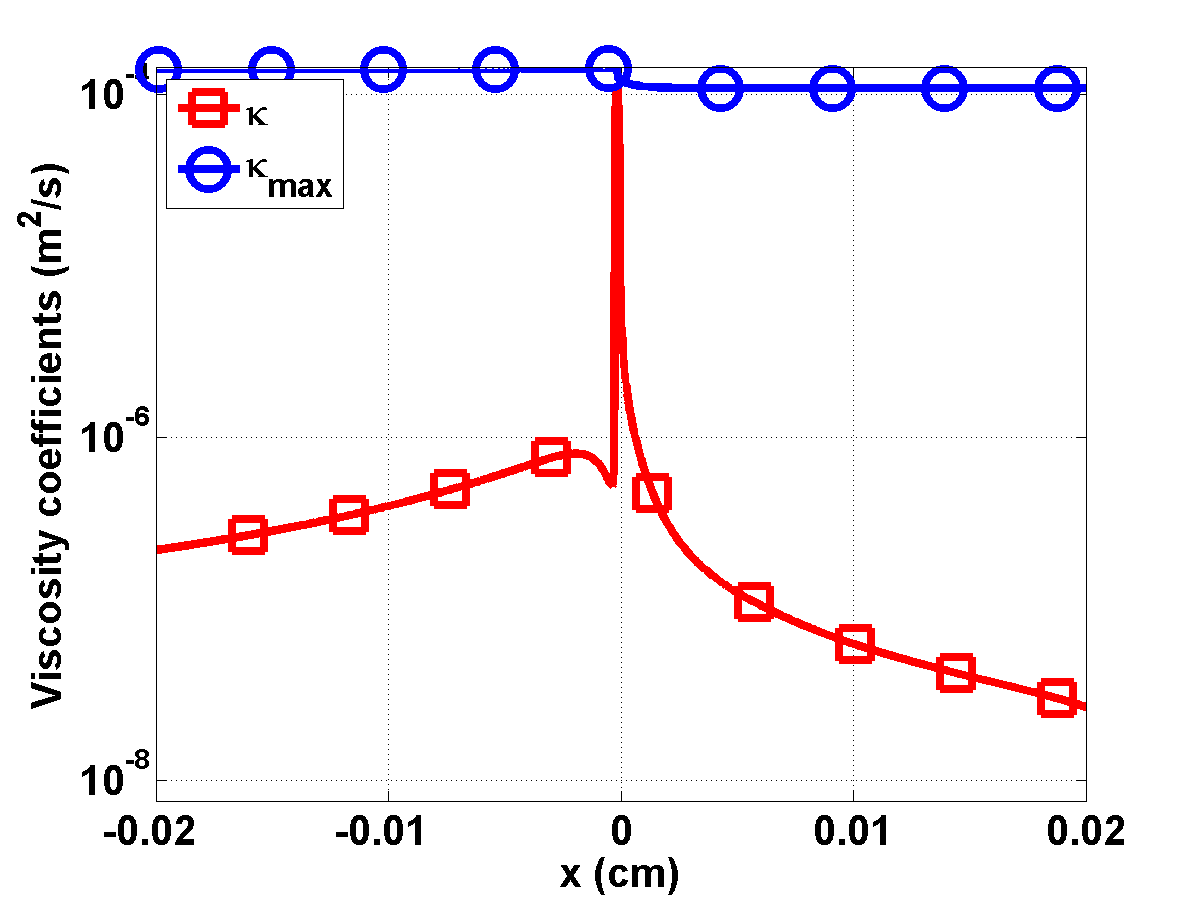
\includegraphics[width=\textwidth]{../elsarticle/Mach_2_nel_2000_viscosity.png}
%                \caption{Density.}
        \end{subfigure}
        \caption{Steady-state numerical solution with $1000$ cells, linear polynomials and BDF2.}
        \end{figure}
\end{frame}
%************************************************
\begin{frame}{Numerical results: Mach $5$.}
\begin{figure}[H]
        \centering
        \begin{subfigure}[b]{0.4\textwidth}
                \centering
                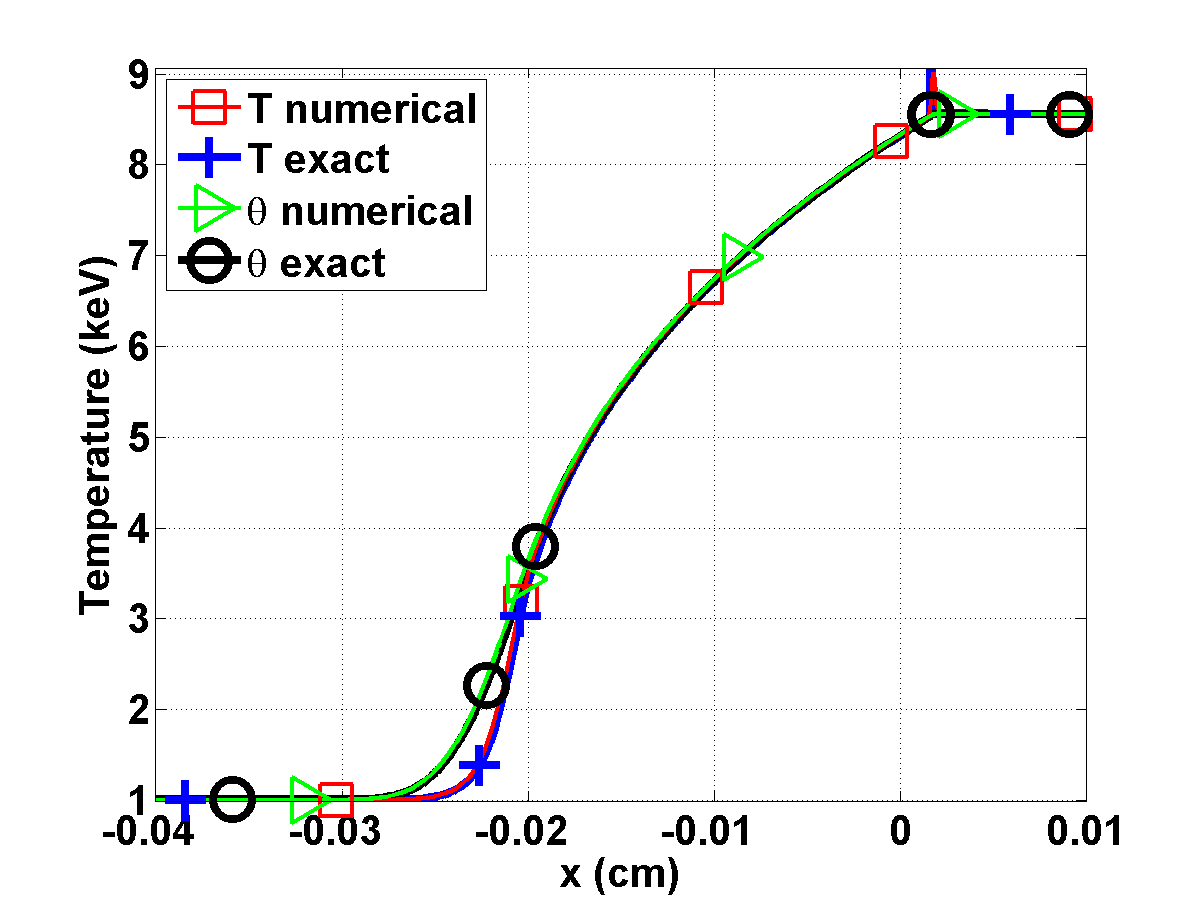
\includegraphics[width=\textwidth]{../elsarticle/Mach_5_nel_2000_temperature.png}
%                \caption{Pressure}
        \end{subfigure}%
        ~ %add desired spacing between images, e. g. ~, \quad, \qquad etc. 
          %(or a blank line to force the subfigure onto a new line)
        \begin{subfigure}[b]{0.4\textwidth}
                \centering
                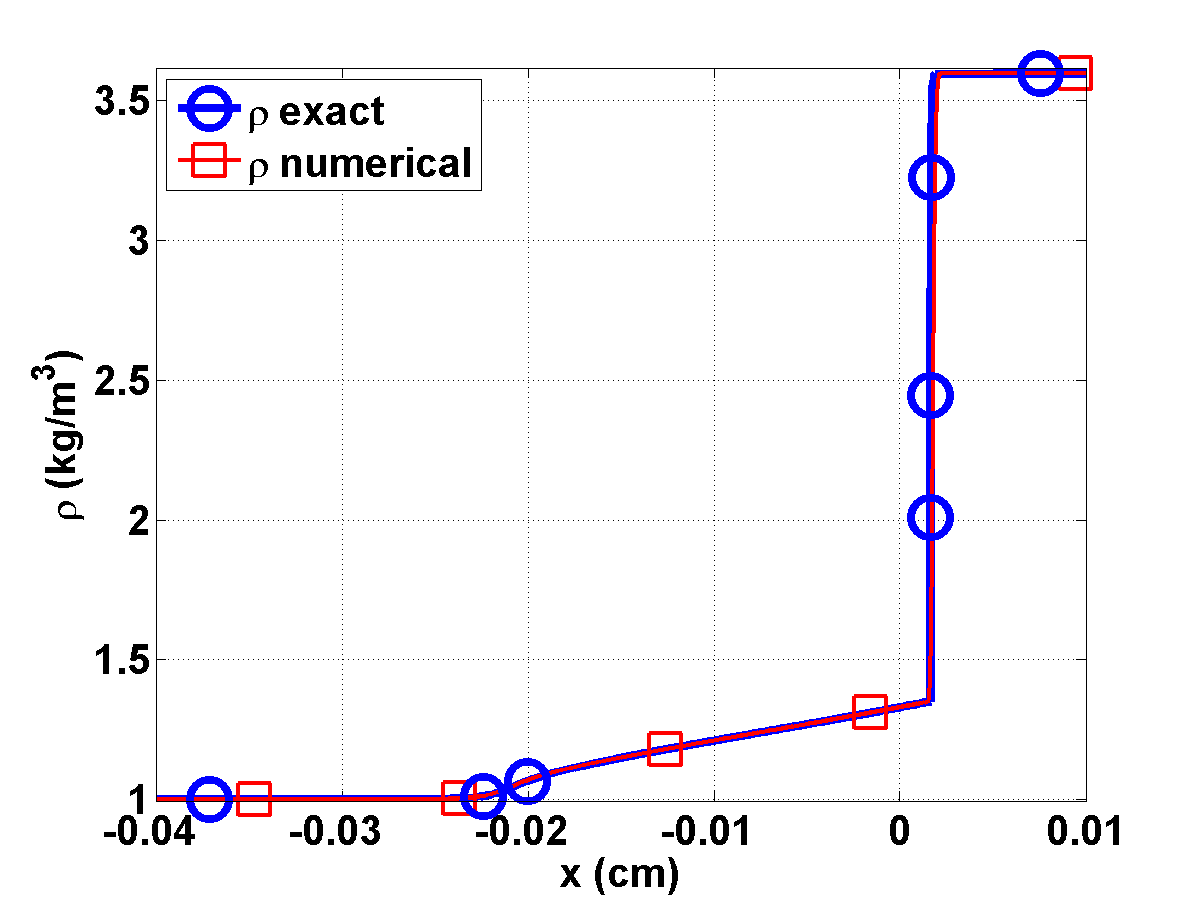
\includegraphics[width=\textwidth]{../elsarticle/Mach_5_nel_2000_density.png}
%                \caption{Velocity.}
        \end{subfigure}
         %add desired spacing between images, e. g. ~, \quad, \qquad etc. 
          %(or a blank line to force the subfigure onto a new line)
        \begin{subfigure}[b]{0.4\textwidth}
                \centering
                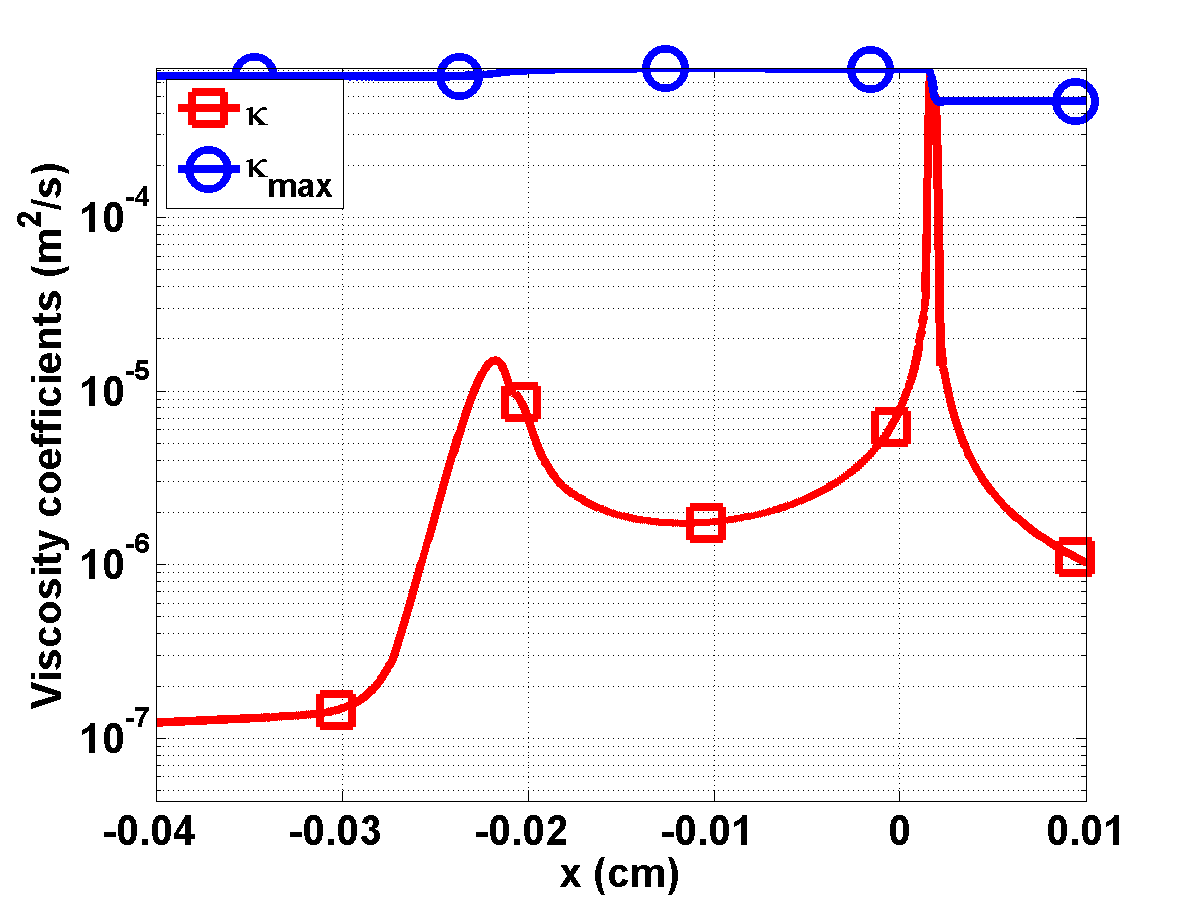
\includegraphics[width=\textwidth]{../elsarticle/Mach_5_nel_2000_viscosity.png}
%                \caption{Density.}
        \end{subfigure}
        \caption{Steady-state numerical solution with $1000$ cells, linear polynomials and BDF2.}
        \end{figure}
\end{frame}
%************************************************
\begin{frame}{Numerical results: Mach $5$, Zeldovich spike.}
\begin{figure}[H]
\centering
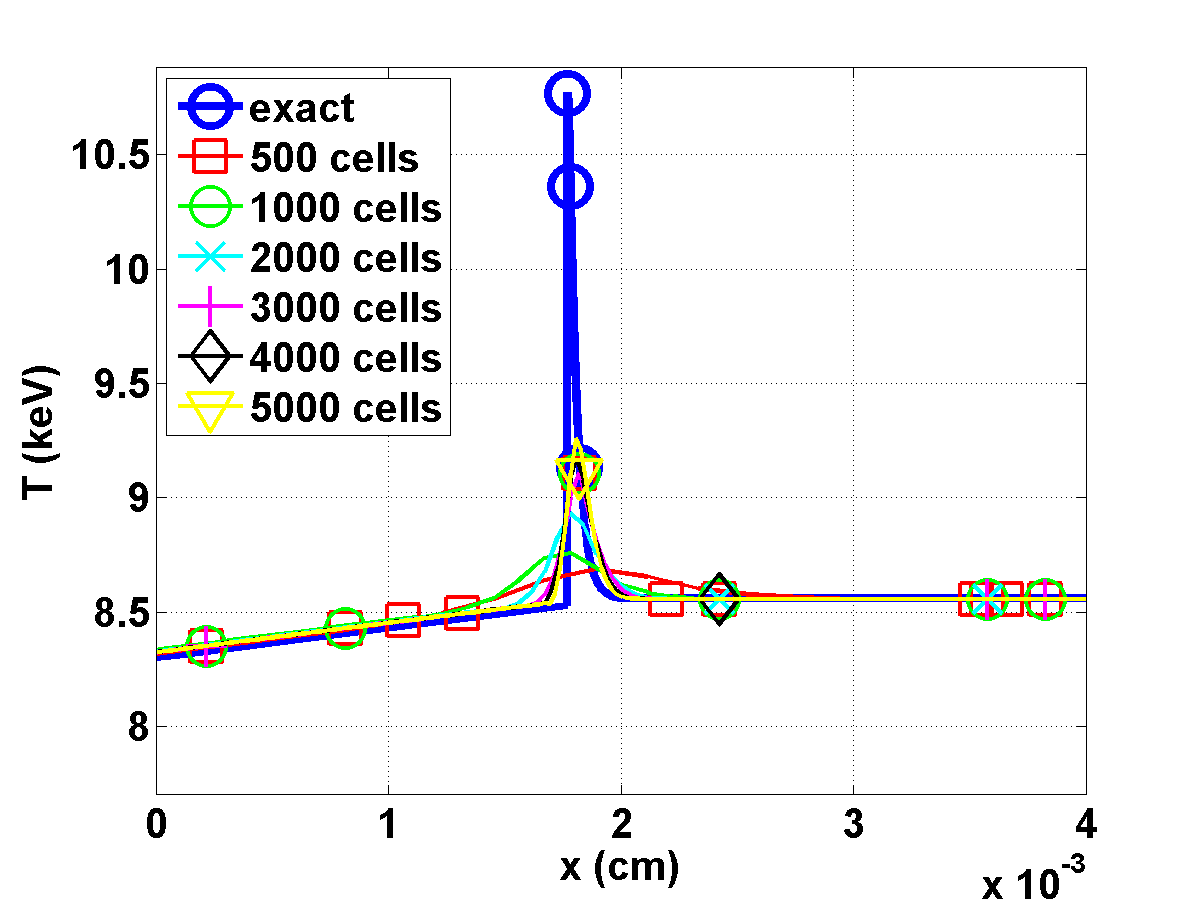
\includegraphics[width=0.8\textwidth]{../elsarticle/Mach_5_comparison.png}
\end{figure}
\end{frame}
%************************************************
\begin{frame}{Numerical results: Mach $50$.}
\begin{figure}[H]
        \centering
        \begin{subfigure}[b]{0.4\textwidth}
                \centering
                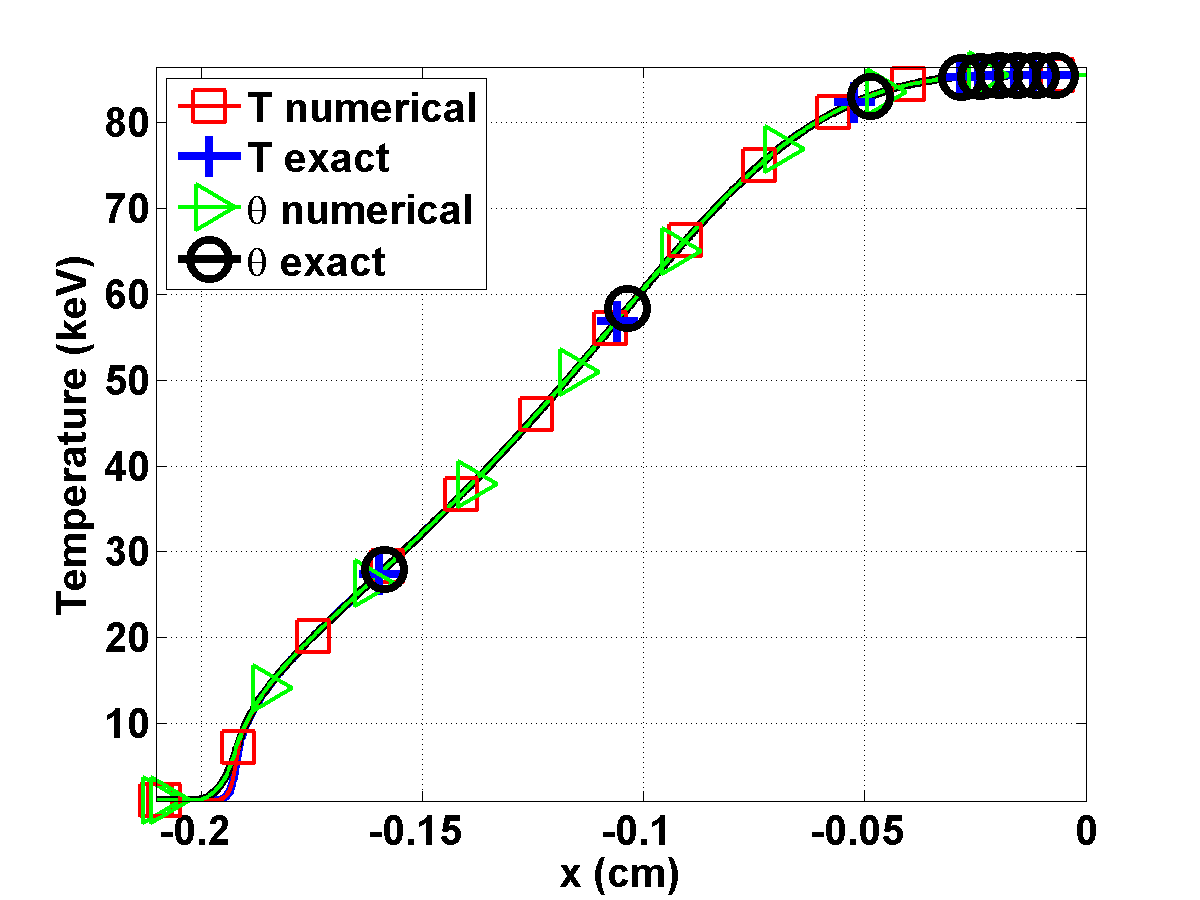
\includegraphics[width=\textwidth]{../elsarticle/Mach_50_nel_1000_temperature.png}
%                \caption{Pressure}
        \end{subfigure}%
        ~ %add desired spacing between images, e. g. ~, \quad, \qquad etc. 
          %(or a blank line to force the subfigure onto a new line)
        \begin{subfigure}[b]{0.4\textwidth}
                \centering
                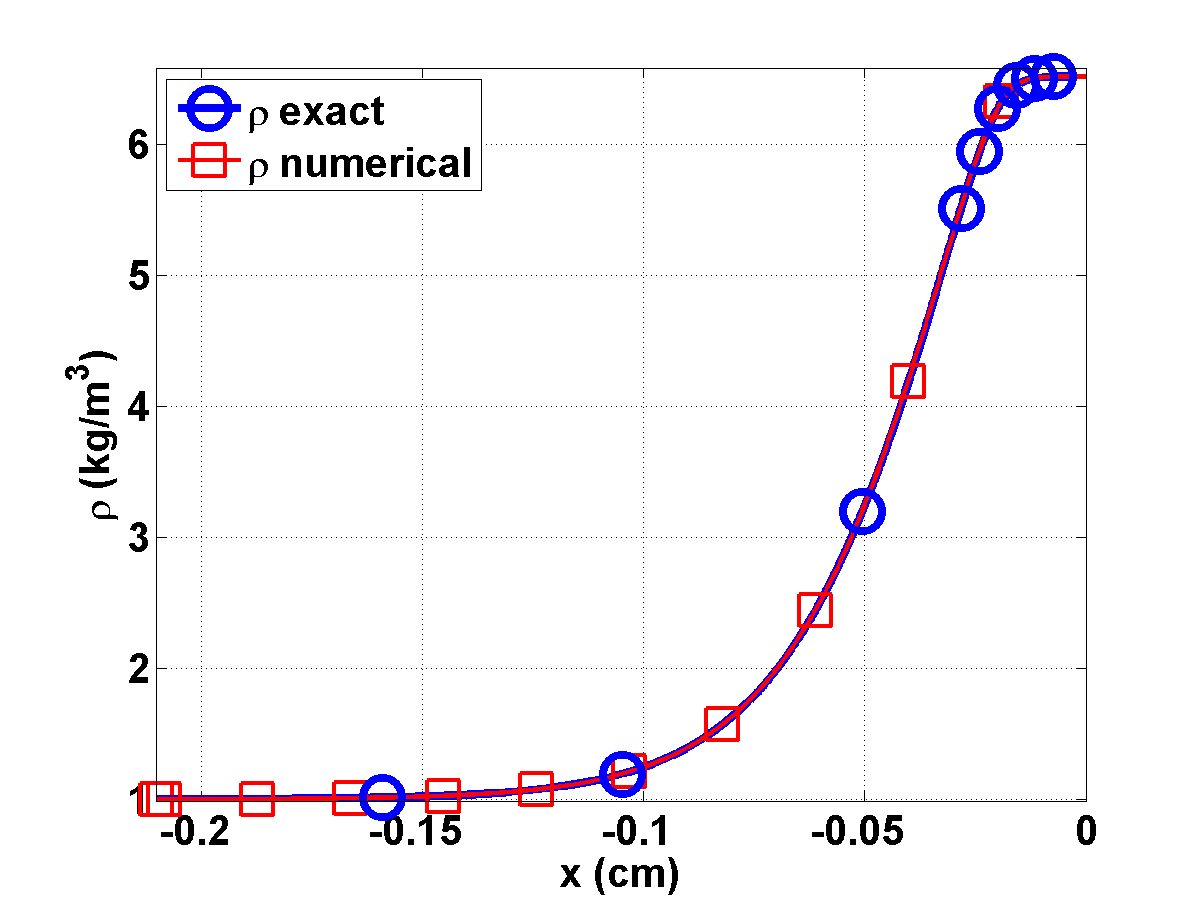
\includegraphics[width=\textwidth]{../elsarticle/Mach_50_nel_1000_density.png}
%                \caption{Velocity.}
        \end{subfigure}
         %add desired spacing between images, e. g. ~, \quad, \qquad etc. 
          %(or a blank line to force the subfigure onto a new line)
        \begin{subfigure}[b]{0.4\textwidth}
                \centering
                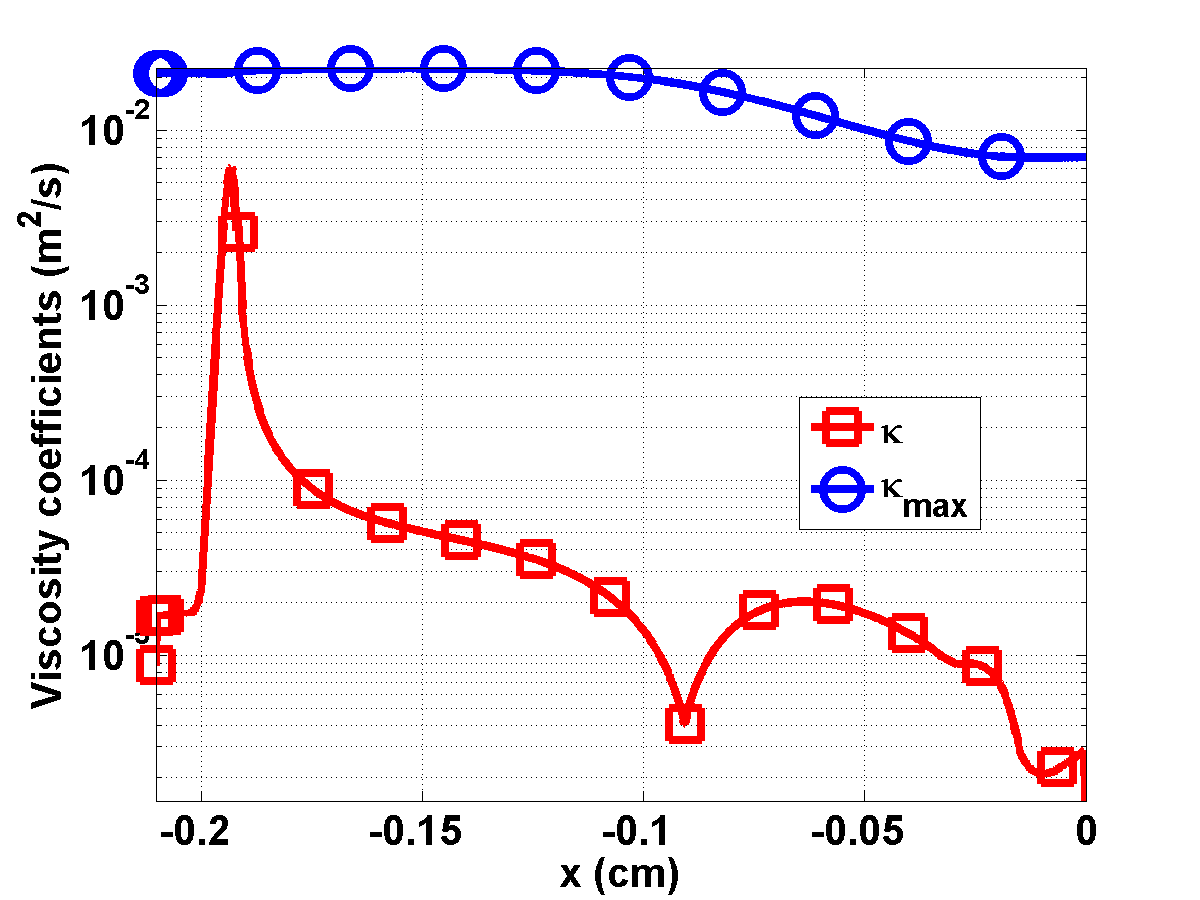
\includegraphics[width=\textwidth]{../elsarticle/Mach_50_nel_1000_viscosity.png}
%                \caption{Density.}
        \end{subfigure}
        \caption{Steady-state numerical solution with $1000$ cells, linear polynomials and BDF2.}
        \end{figure}
\end{frame}
%************************************************
\section{Conclusions and future work.}
\begin{frame}
\begin{block}{Conclusions:}
\begin{itemize}
\setlength{\itemsep}{14pt}
\item The entropy viscosity method was successfully applied to the $1$-D RHD.
\item $1$-D numerical results show good agreement with semi-analytical solutions.
\item Demonstrated high-order accuracy and correct behavior in the equilibrium diffusion limit.
\item The method can be applied with any equation of state with a convex entropy.
\item The method is simple to implement and the viscosity coefficient is computed on the fly.
\end{itemize}
\end{block}
\begin{block}{Future work:}
\begin{itemize}
\setlength{\itemsep}{14pt}
\item Extension to multi-D simulations: the theoretical approach holds.
\item $S_n$ transport approximation (instead of the radiation-diffusion equation) coupled to Euler equations.
\end{itemize}
\end{block}
\end{frame}
%************************************************
\begin{frame}{}
\begin{center}
\LARGE{\textbf{QUESTIONS/COMMENTS ?}}
\end{center}
\end{frame}
%************************************************
%************************************************
%************************************************
\begin{frame}{Entropy residual with dissipative terms:}
\begin{block}{}
 \begin{align}
 \frac{Ds}{Dt} + \underbrace{\left( P \partial_e s + \rho^2 \partial_{\rho} s + \frac{4}{3} \rho \epsilon \partial_{\epsilon} s \right) \partial_x u}_\text{(a)} &= \nonumber\\
 \partial_x \left( \rho \kappa \partial_x s \right) &+ \kappa \partial_e s \partial_x s - \rho \kappa \underbrace{X A X^t}_\text{(b)} + \underbrace{ s_e \rho \mu (\partial_x u)^2}_\text{(c)} \nonumber
 \end{align}
 \end{block}
 \begin{block}{}
 where $X$ is a row vector defined as $X=\left( \rho, e, \epsilon \right)$ and $A$ is the $3$x$3$ symmetric matrix:
 \begin{equation}
 A = 
 \left[
 \begin{array}{ccc}
\partial_{\rho} \left( \rho^2 \partial_{\rho} s \right) & \partial_{\rho,e} s & \partial_{\rho} \left( \rho \partial_{\epsilon} s \right) \\
 \partial_{\rho,e} s & \partial_{e,e} s & \partial_{e,\epsilon} s \\
 \partial_{\rho} \left( \rho \partial_{\epsilon} s \right) & \partial_{e,\epsilon} s & \partial_{\epsilon,\epsilon} s
 \end{array}
 \right] \nonumber
 \end{equation}
 \end{block}
\end{frame}
%************************************************
\begin{frame}{Positivity of the matrix $A$:}
\begin{block}{}
With $s(\rho, e, \epsilon) = \tilde{s}(\rho,e) + \frac{\rho_0}{\rho}\hat{s}(\epsilon)$:
 \begin{equation}
 A = 
 \left[
 \begin{array}{ccc}
\partial_{\rho} \left( \rho^2 \partial_{\rho} \tilde{s} \right) & \partial_{\rho,e} \tilde{s} & 0 \\
 \partial_{\rho,e} \tilde{s} & \partial_{e,e} \tilde{s} & 0 \\
 0 & 0 & {\color{blue}\rho^{-1} \partial_{\epsilon,\epsilon} \hat{s}}
 \end{array}
 \right] \nonumber
 \end{equation}
\end{block}
\end{frame}
%************************************************
%************************************************
%************************************************
%************************************************
\begin{frame}[allowframebreaks]
\bibliographystyle{apalike}
\bibliography{Biblio-Database}
\begin{thebibliography}{47}
  
  \bibitem{jlg1}
  {\em Entropy viscosity method for nonlinear conservation laws}, 
  Jean-Luc Guermond, R. Pasquetti, B. Popov, J. Comput. Phys., 230 (2011) 4248-4267.
  
  \bibitem{jlg2}
  {\em Entropy Viscosity Method for High-Order Approximations of Conservation Laws}, 
  J-L. Guermond, R. Pasquetti, 
  Lecture Notes in Computational Science and Engineering, Springer, Volume 76, (2011) 411-418.

 \bibitem{jlg3}
 \emph{Entropy-based nonlinear viscosity for Fourrier approximations of conservation laws}, 
 J.-L. Guermond, R. Pasquetti, C.R. Math. Acad. Sci. Paris 346 (2008) 801�806.
  
  \bibitem{Balsara}
  \emph{An Analysis of the Hyperbolic Nature of the Equations of Radiation Hydrodynamics},
  Dinshaw S. Balsara, J. Quant. Spectrosc. Radiat. Transfer, Vol. 61, No. 5, pp. 617-627, 1999.
  
  \bibitem{LowrieMorelHittinger}
  \emph{The coupling of radiation and hydrodynamics},
  Lowrie RB, Morel JE, Hittinger JA, 521 (1), 432-50 (1999).

  \bibitem{FluxLimiter1}
  \emph{Advanced numerical approximation of nonlinear hyperbolic equations}, 
  B. Cockburn, C. Johnson, C. Shu, E. Tadmor, Lecture Notes in Mathematics, vol. 1697, Springer, 1998.
  
  \bibitem{FluxLimiter2}
  \emph{Discontinuous Galerkin methods: theory, computation and applications}, 
  B. Cockburn, G. Karniadakis, C. Shu, Lecture Notes in Computer Science and Engineering, vol. 11, Springer, 2000.
  
  \bibitem{FluxLimiter3}
  \emph{The local discontinuous Galerkin method for time- dependent convection-diffusion systems}, 
  B. Cockburn, C. Shu, SIAM J. Numer. Anal. 35 (1998) 2440�2463.
  
\bibitem{FluxLimiter4}
\emph{New non-oscillatory central schemes on unstructured triangulations for hyperbolic systems of conservation laws}, 
I. Christov, B. Popov, J. Comput. Phys. 227 (11) (2008) 5736�5757.

\bibitem{EdwardsMorelKnoll}
 \emph{Nonlinear variants of the TR$-$BDF$2$ method for thermal radiative diffusion},
 Jarrods D. Edwards, Jim E. Morel, Dana A. Knoll, Journal of Computational Physics, 230 (2011), 1198-1214.
 
  \bibitem{Toro}
  \emph{Riemann Solvers and numerical methods for fluid dynamics.}
  E.F. Toro, $2^{nd}$ Edition, Springer.  
  
  \bibitem{Reisner}
  \emph{A space-time smooth artificial viscosity method for nonlinear conservation laws}
  Reisner J., Serencsa J. and Shkoller S., Journal of Computational Physics 235 (2013) 912-933.
    
  \bibitem{LowrieMorel}
  \emph{Issues with high-resolution Godunov methods for radiation hydrodynamics},
  R.B. Lowrie, J.E. Morel, Journal of Quantitative Spectroscopy \& Radiative Transfer, 69, 475-489 (2001).

\bibitem{EdwardsMorelLowrie}
\emph{Second-Order Discretization in Space and Time for Radiation Hydrodynamics},
Jarrod D. Edwards, Jim E. Morel, Robert B. Lowrie, International Conference on Mathematics and Computational Methods Applied to Nuclear Science \& Engineering (M\&C 2013), Sun Valley, Idaho USA, May 5-9, American Nuclear Society, LaGrange Park, II (2013).
   
  \bibitem{ShiJin}
  \emph{Numerical Schemes for Hyperbolic Conservation Laws with Stiff Relaxation Terms}, 
  Shi Jin and C. David Levermore, Journal of Computational Physics, 126, 449-467 (1996).
  
  \bibitem{jlg}
  \emph{Viscous regularization of the Euler equations and entropy principles},
  Jean-Luc Guermond and Bojan Popov, under review.
  
  \bibitem{Moose}
  \emph{A parallel computational framework for coupled systems of nonlinear equations},
  D. Gaston, C. Newsman, G. Hansen and D. Lebrun-Grandie, Nucl. Eng. Design, vol 239, pp 1768-1778, 2009.
  
  \bibitem{RatTherm}
  \emph{Rational thermodynamics},
  Truesdell C. and Wang C.-C., New York, McGraw-Hill Book Company, 1969, XII. 208 S.
  
  \bibitem{IGEOS}
  \emph{A to Z of Thermodynamics},
  Perrot P., Oxford University Press (1998).
  
  \bibitem{PBV_book}
  \emph{Applied CFD Techniques: an Introduction based on Finite Element Methods},
  Rainald Lohner, $2^{nd}$ Edition, Wiley.
  
  \bibitem{Leblanc}
  \emph{Validation Test Case Suite for compressible hydrodynamics computation},
  Loubere R., Theoritical Division, T-7, Los Alamos National Laboratory (pdf version).
  
\end{thebibliography}
\end{frame}
%-------------------------------------------------------------------------------------------------------------------
\end{document}

